\chapter{Windows}

\section{取消windows的管理员权限提示}

打开组策略编辑器,定位到计算机配置—windows设置—安全设置—本地策略
—安全选项,然后将“用户帐户控制:管理员批准模式中管理员的提升权限提示的行为”
进行修改为“不提示,直接提升”,如下图:
\begin{figure}[H]
  \centering
  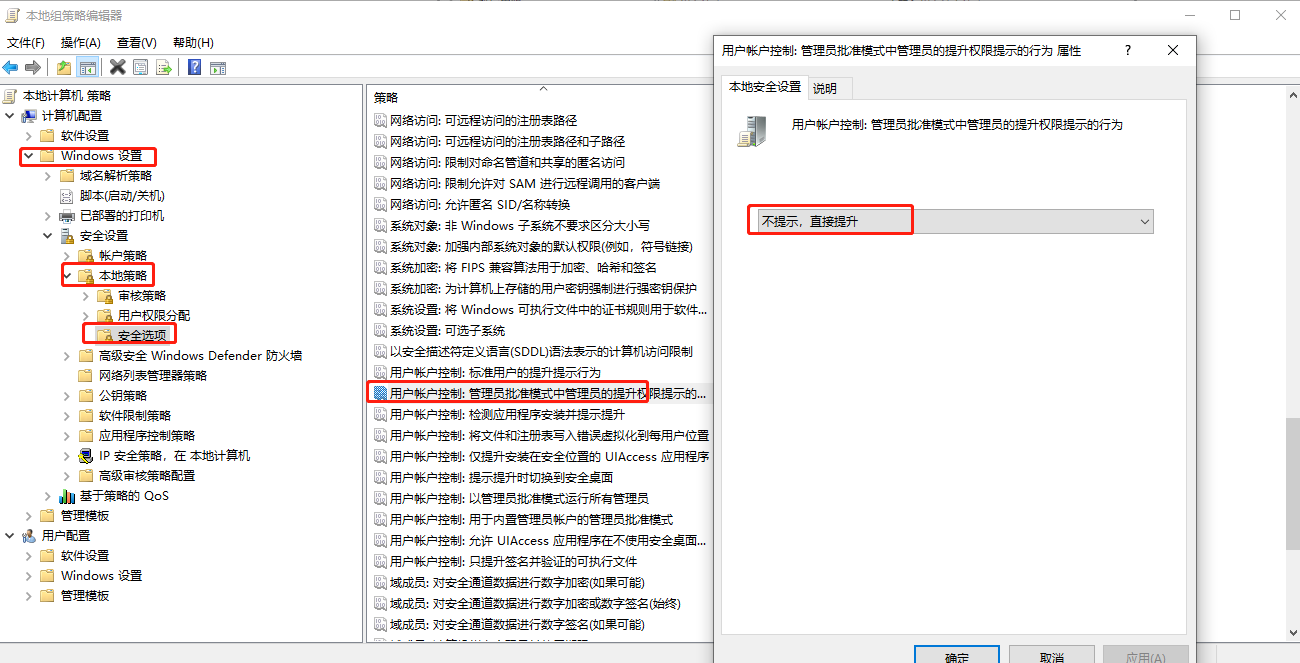
\includegraphics[width=\linewidth]{windows_admin.png}
  \caption{取消windows的管理员权限提示}
  \label{fig:windows_admin}
\end{figure}

\section{Danbooru图站的高级搜索}
Danbooru图站支持多种搜索条件,可以用于精确搜索

\begin{code-block}{bash}

#按照分辨比例
# ratio后可以为>,<等比较符
ratio:4:3

#按照高度
width:100

#按照宽度
height:100

#宽屏优先
order:landscape

#竖屏优先
order:portrait
\end{code-block}

\section{修改windows下的ssh-key的权限问题}
将ssh-key放到\codeinline{powershell}{C:\Users\\zhangjl\.ssh}下,然后用管理员权限打开powershell,执行如下
命令即可:
\begin{code-block}{powershell}
# Set Key File Variable:
New-Variable -Name Key -Value "$env:UserProfile\.ssh\id_rsa"
# Remove Inheritance:
Icacls $Key /c /t /Inheritance:d

# Set Ownership to Owner:
# Key's within $env:UserProfile:
Icacls $Key /c /t /Grant ${env:UserName}:F

# Key's outside of $env:UserProfile:
TakeOwn /F $Key
Icacls $Key /c /t /Grant:r ${env:UserName}:F

# Remove All Users, except for Owner:
Icacls $Key /c /t /Remove:g Administrator "Authenticated Users" BUILTIN\Administrators BUILTIN Everyone System Users

# Verify:
Icacls $Key

# Remove Variable:
Remove-Variable -Name Key
\end{code-block}

\section{Windows WSL的权限}
\begin{code-block}{bash}
cat >>~/.bashrc<<EOF
if [[ "$(umask)" == '000' ]]; then
    umask 022
fi
EOF

cat > /etc/wsl.conf<<EOF
[automount]
enabled = true
root = /mnt/
options = "metadata,dmask=022,fmask=133"
mountFsTab = false
EOF
\end{code-block}

然后重启windows即可。同时,也可以实现在wsl下挂载iso/windows磁盘的功能:
\begin{code-block}{bash}
# 将windows的E盘/虚拟光驱挂载到/srv下
mount -t drvfs E: /srv
\end{code-block}
